% vim: set tw=78 tabstop=4 shiftwidth=4 aw ai:
\documentclass{beamer}

\usepackage[utf8x]{inputenc}		% diacritice
\usepackage[english]{babel}
\usepackage{color}			% highlight
\usepackage{alltt}			% highlight
\usepackage{caption}
\usepackage{frame}
\usepackage{listings}

\lstset{language=Java,
    basicstyle=\ttfamily,
    showspaces=true,
    numbers=left,
}


\usepackage{hyperref}			% folosiți \url{http://...}
					% sau \href{http://...}{Nume Link}
\usepackage{verbatim}

\mode<presentation>
{ \usetheme{Berlin} }

% Încărcăm simbolurilor Unicode românești în titlu și primele pagini
\PreloadUnicodePage{200}

% Arătăm numărul frame-ului
\newcommand{\frameofframes}{/}
\newcommand{\setframeofframes}[1]{\renewcommand{\frameofframes}{#1}}

\setframeofframes{of}
\makeatletter
\setbeamertemplate{footline}
  {%
    \begin{beamercolorbox}[colsep=1.5pt]{upper separation line foot}
    \end{beamercolorbox}
    
    \begin{beamercolorbox}[ht=2.5ex,dp=1.125ex,%
      leftskip=.3cm,rightskip=.3cm plus1fil]{title in head/foot}%
      {\usebeamerfont{title in head/foot}\insertshorttitle}%
      \hfill%
      {\usebeamerfont{frame number}\usebeamercolor[fg]{frame number}\insertframenumber~\frameofframes~\inserttotalframenumber}
    \end{beamercolorbox}%
    \begin{beamercolorbox}[colsep=1.5pt]{lower separation line foot}
    \end{beamercolorbox}
  }
\makeatother

\setbeamertemplate{navigation symbols}{}%remove navigation symbols

\title[Deep Learning Models for Games]{Deep Learning Models for Games}
\subtitle{Bachelor Thesis Session -- September 2015}
\institute{Faculty of Automatic Control and Computers,\\
	University POLITEHNICA of Bucharest}
\author[Florentina-Ștefania Bratiloveanu]{Florentina-Ștefania Bratiloveanu\\
	Supervisor: As. Drd. Ing Tudor Berariu}
\date{September 14, 2015}

\begin{document}

% Slide-urile cu mai multe părți sunt marcate cu textul (cont.)
\setbeamertemplate{frametitle continuation}[from second]

\frame{\titlepage}

\frame{\tableofcontents}

% NB: Secțiunile nu sunt marcate vizual, ci doar apar în cuprins


%--------------------MOTIVATION--------------------	
\section{Motivation}
\begin{frame}{Motivation}
	\begin{Huge}
		Deep Learning
	\end{Huge}
	\vspace*{0.8cm}
	\begin{itemize}
	
		\item find models capable of generalization
		\item extract from low-level(edges,colors) to high-level(combination of rudimentary features) features
		\item reduce programming burden
		\item applicability: cancer classification, autonomous cars, object recognition from images
	\end{itemize}
\end{frame}

\section{State of the art}
%--------------------INTRODUCTION--------------------	
\begin{frame}{Once upon a time...}
	\begin{itemize}
		\item reinforcement learning: Q-Learning
		\item deep neural networks
	\end{itemize}
	\begin{center}
		\includegraphics[width=205px,height=130px]{img/nn2}
	\end{center}
	
\end{frame}

%--------------------PREPROCESSING, MODEL, LOSS FUNCTION--------------------	
\begin{frame}{Preprocessing, Model, Loss function}
	\begin{itemize}
		\item color space: RGB, YUV, grayscale
		\item data normalization 0..1, contrast normalization
		\item activation functions
		\begin{itemize}
			\item hidden layer vs output layer
			\item tanh, sigmoid, ReLU
		\end{itemize}
		\item how many layers/features, what type of layers
		\item loss function: classification(binary/multi-class) or regression?
		\item gradient descent \textbf{vs} stochastic gradient descent
	\end{itemize}
\end{frame}

%--------------------TRAINING AND TESTING--------------------	
\begin{frame}{Train and test}
	\begin{itemize}
		\item split dataset for training and testing
		\item when to stop training?
	\end{itemize}
	 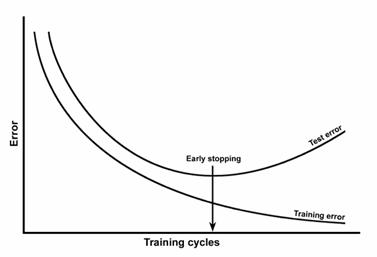
\includegraphics[width=180px,height=123px]{img/traintest.jpg}
	 \begin{flushleft}
	 
			\fontsize{5}{1em}{\texttt{Source:}} \\
			\vspace*{-0.2cm}			
			\fontsize{4}{1em}{\texttt{
			\url{http://documentation.statsoft.com/statisticahelp.aspx?path=sann/overview/sannoverviewsnetworkgeneralization}}}
	\end{flushleft}
\end{frame}

\section{Architecture, Design, Results}
\begin{frame}{Once upon a time...}
	\begin{minipage}{0.5\textwidth}
		\begin{figure}[H]
			\fbox{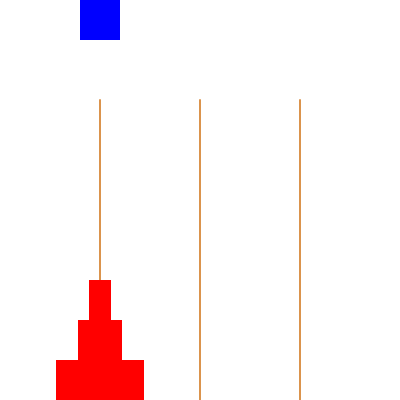
\includegraphics[width=60px,height=60px]{img/155}}
			\caption*{Tower of Hanoi (first state)}
		\end{figure}
		\vspace*{-1.45cm}
		\begin{figure}[H]
			\centering
			\captionsetup{justification=centering}
			\fbox{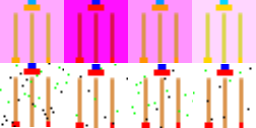
\includegraphics[width=154px,height=77px]{img/states}}
			\caption*{Dataset with noise added and color changed}
		\end{figure}
	\end{minipage} \hfill
	\begin{minipage}{0.45\textwidth}
		\begin{itemize}
			\item game: Tower of Hanoi
			\item reinforcement learning: Q-Learning
			\item deep neural networks: predict values from Q-Learning
			\item machine learning framework: Torch based on Lua
		\end{itemize}
	\end{minipage}
\end{frame}


\begin{frame}{Q-Learning}
	\begin{itemize}
		\item finds optimal policy for action-value function
		\item 
		Q(s,a) = Q(s,a) + $\alpha\cdot$(r + $\gamma\cdot \max_a Q(s^\prime,a^\prime)-Q(s,a)$)
	\end{itemize}	
	\begin{figure}[hp]
		\centering
		\minipage{0.30\textwidth}
  			\framebox{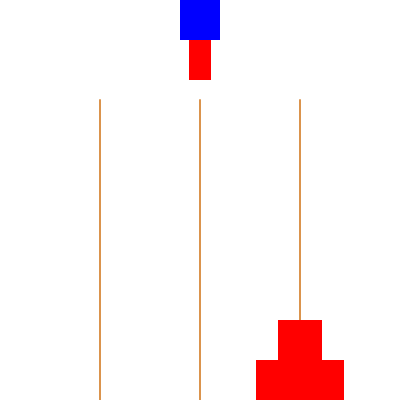
\includegraphics[width=\linewidth]{img/50}}
  			\caption*{\scriptsize{\newline UP = 90,6534\newline DOWN = 86,8787\newline LEFT = 89,1867\newline RIGHT = 94,2824}}\label{fig:fa}
		\endminipage\hfill
		\minipage{0.30\textwidth}
  			\framebox{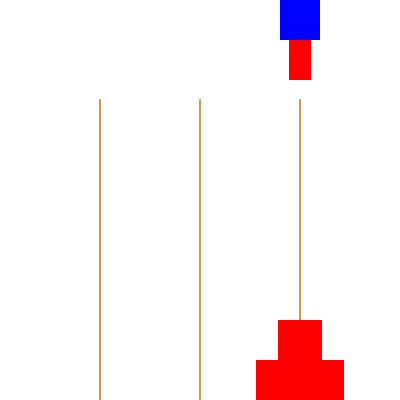
\includegraphics[width=\linewidth]{img/85}}
  			\caption*{\scriptsize{\newline UP = 97,6530\newline DOWN = 100,0000\newline LEFT = 93,8538\newline RIGHT = 92,5261}}\label{fig:fb}
		\endminipage\hfill
		\minipage{0.30\textwidth}%
 			\framebox{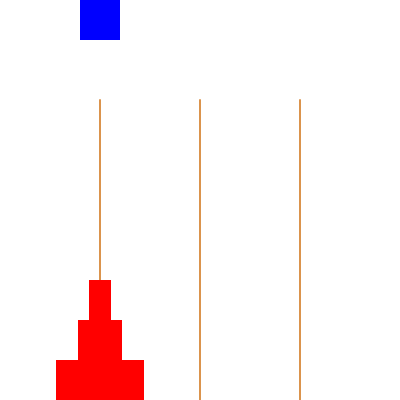
\includegraphics[width=\linewidth]{img/155}}
   			\caption*{\scriptsize{\newline UP = 26,3520\newline DOWN = 23,8452\newline LEFT = 23,8897\newline RIGHT = 22,8827}}\label{fig:fc}
		\endminipage
	\end{figure}
\end{frame}



\subsection{Regression with complex model}
\begin{frame}{Model}
	\begin{center}
		\hspace*{-0.7cm}
		\includegraphics[width=345px,height=93px]{img/complex}
    \end{center}
\end{frame}

\begin{frame}{Results}
	\begin{center}
		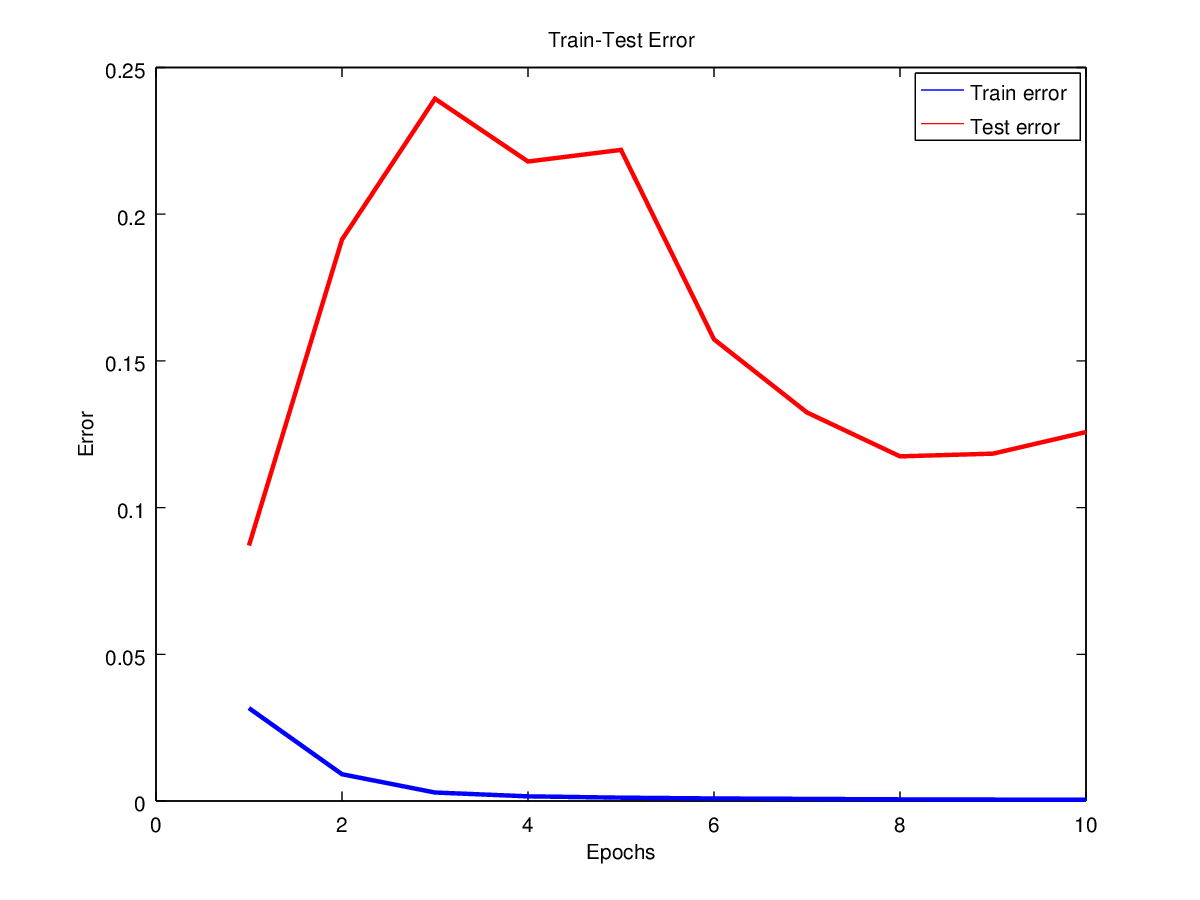
\includegraphics[width=240px,height=180px]{img/train-test-100}
    \end{center}
\end{frame}


\subsection{Regression with simple model}
\begin{frame}{Model}
	\begin{center}
		\hspace*{-0.6cm}
		\includegraphics[width=338px,height=126px]{img/simple}
    \end{center}
\end{frame}

\begin{frame}{Results}
\begin{figure}[h]
	\begin{center}
		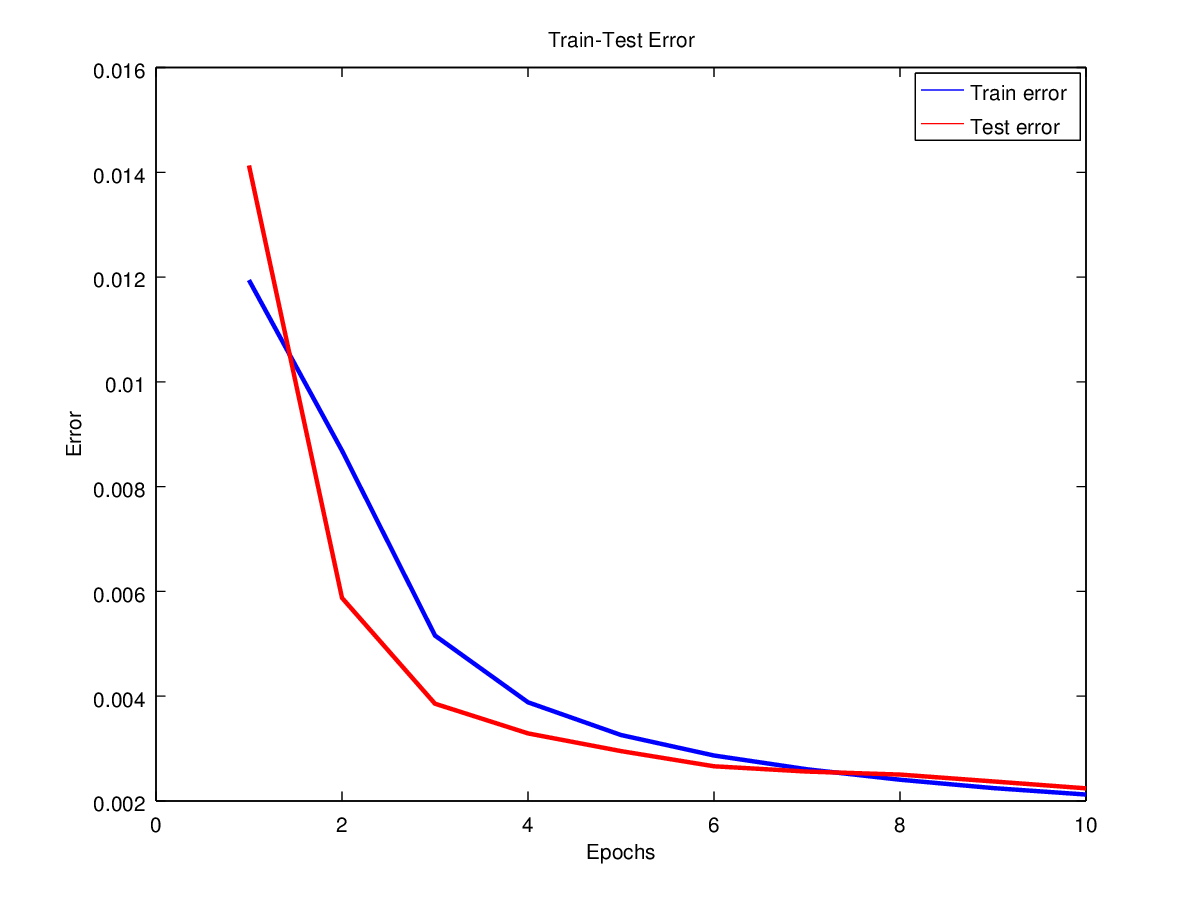
\includegraphics[width=240px,height=180px]{img/small-network}
    \end{center}
\end{figure}

\end{frame}

%--------------------FUTURE WORK--------------------	
\section{Future work}
\begin{frame}{Future work}
	\begin{itemize}
		\item implement Q-Network
		\item test algorithm on dynamic environments or games where the state of the universe is not fully observed
		\item make Nao capable of playing Tic-Tac-Toe
		\item after all tasks mentioned above are done, use all the information gathered for cancer classification, etc.
	\end{itemize}
\end{frame}

%--------------------CONCLUSIONS--------------------
\section{Conclusions}
\begin{frame}{Conclusions}
\begin{figure}[h]  
	\begin{minipage}[b]{0.3\textwidth}    
		
\includegraphics[width=\textwidth]{img/joke}
  	\end{minipage}
  	\hfill
  	\begin{minipage}[t]{0.55\textwidth}
		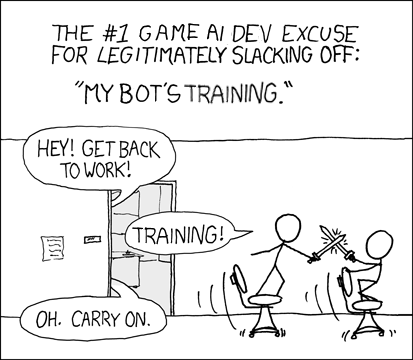
\includegraphics[width=\textwidth]{img/training}	   
	\end{minipage}
\end{figure}
\begin{flushright}
			\fontsize{5}{1em}{\texttt{Source:}} \\
			\vspace*{-0.2cm}			
			\fontsize{4}{1em}{\texttt{
			\url{http://xkcd.com/}}}
\end{flushright}	
\end{frame}

%--------------------QUESTIONS--------------------
\section{QA}
\begin{frame}{QA}
	\begin{center}
    \bfseries
    \large
    Questions and Answers
    
    \vspace*{1.9cm}			
    Thank you for your attention!
  	\end{center}
\end{frame}


\end{document}
